\begin{question}{22}{
    In a joint project between physical training instructors of the Royal Military Academy (KMA) and the medical service, the relationship is investigated
    between average sleep duration of a cadet (in hours) and the recovery time after intense physical exertion (in hours).
    
    Recovery time is measured using a muscle soreness index; a cadet is considered fully recovered when this index falls below a certain threshold.

    Voor de hersteltijd wordt gekeken naar een spierpijn-index, en een cadet is volledig hersteld wanneer de spierpijn-index onder een gegeven drempelwaarde komt.

    For nine cadets, the average sleep duration and recovery time after intense exertion are measured.
    \begin{center}
        \begin{tabular}{c|ccccccccc}
            \toprule
                \textbf{Sleep duration (in hours)} & $4,0$ & $4,5$ & $5,0$ & $5,5$ & $6,0$ & $6,5$ & $7,0$ & $7,5$ & $8,0$ \\
                \textbf{Recovery time (in hours)} & $66$ & $61$ & $63$ & $62$ & $65$ & $64$ & $57$ & $59$ & $60$ \\
            \bottomrule
        \end{tabular}
    \end{center}
}
    
    \subquestion{2}{
        If we want to perform a regression analysis, which variable would be the dependent variable $Y$ and which variable the independent variable $X$?
    }
    \solution{
        In regression analysis, it makes the most sense to take sleep time as the independent variable $X$ and recovery time as the dependent variable $Y$.
        A longer recovery time does not explain why someone sleeps longer, but the other way around might make sense.\rubric{2}
    }
    \subquestion{5}{
        Draw the corresponding scatter plot based on your answer to subquestion (a).
    }
    \solution{
        \begin{center}
            \resizebox{0.9\textwidth}{!}{
                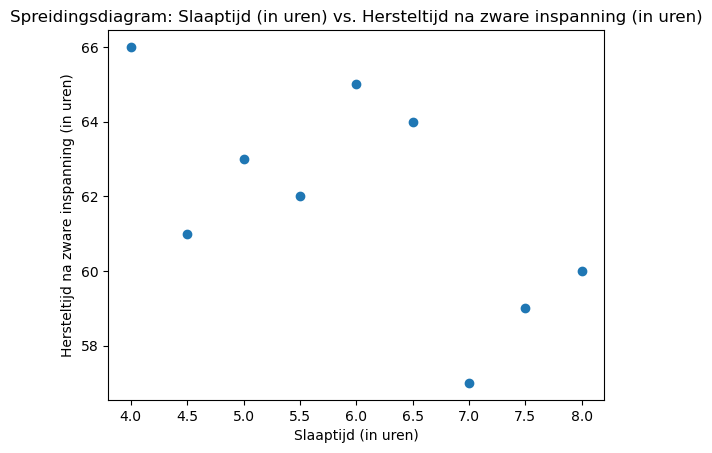
\includegraphics{20250725_q4_scatterplot.png}
            }
        \end{center}
    }

    \subquestion{8}{
        Calculate Pearson's correlation coefficient $r(x,y)$.
        What can you conclude about the relationship between the two variables?
    }
    \solution{
        We start by calculating Pearson's correlation coefficient:
        \begin{align*}
            r(x, y) = \frac{\overline{xy} - \overline{x} \cdot \overline{y}}{\sqrt{(\overline{x^2} - \overline{x}^2)\cdot(\overline{y^2} - \overline{y}^2) }}
        \end{align*}
        We use the following table to find the necessary values:
        \begin{center}
            \begin{tabular}{ccccc}
                \toprule
                    $x$ & $y$ & $xy$ & $x^2$ & $y^2$ \\
                \midrule
    		        $4$ & $66$ & $264$ & $16$ & $4356$ \\
                    $4,5$ & $61$ & $274,5$ & $20,25$ & $3721$ \\
                    $5$ & $63$ & $315$ & $25$ & $3969$ \\
                    $5,5$ & $62$ & $341$ & $30,25$ & $3844$ \\
                    $6$ & $65$ & $390$ & $36$ & $4225$ \\
                    $6,5$ & $64$ & $416$ & $42,25$ & $4096$ \\
                    $7$ & $57$ & $399$ & $49$ & $3249$ \\
                    $7,5$ & $59$ & $442,5$ & $56,25$ & $3481$ \\
                    $8$ & $60$ & $480$ & $64$ & $3600$ \\
                \midrule
                    $\overline{x} = 6$ & $\overline{y} = 61,8889$ & $\overline{xy} = 369,1111$ & $\overline{x^2} = 37,6667$ & $\overline{y^2} = 3837,8889$ \\
                \bottomrule
            \end{tabular} \rubric{4}
        \end{center}
        Now we compute Pearson's correlation coefficient as follows:
        \begin{align*}
            r(x,y)  &= \frac{ \overline{x \cdot y} - \overline{x} \cdot \overline{y} }{ \sqrt{ (\overline{x}^2 - \overline{x^2}) \cdot (\overline{y}^2 - \overline{y^2}) } }\\
                    &= \frac{ 369,1111 - 6 \cdot 61,8889 }{ \sqrt{ (6^2 - 37,6667) \cdot (61,8889^2 - 3837,8889) } } \\
                    &= \frac{-2,2222}{3,5717} \\
                    &\approx -0,6222.\rubric{3}
        \end{align*}
        The correlation coefficient is clearly negative and not close to zero, indicating a fairly strong negative trend.
        However, there is still some uncertainty in the exact linear relationship. \rubric{1}
    }

    \subquestion{7}{
        Calculate the regression line $Y = a + b \cdot X$ by computing the coefficients $a$ and $b$.
        Based on this regression line, give a statistically sound prediction for the recovery time of a cadet who has slept for $6$ hours and $45$ minutes.
    }
    \solution{
        In order to compute the coefficients $a$ and $b$, we reuse the table from subquestion (a).
        We have that
        \begin{align*}
            b &= \frac{\overline{xy} - \overline{x} \cdot \overline{y}}{\overline{x^2} - (\overline{x})^2} \\
              &= \frac{369,1111 - 6 \cdot 61,8889}{37,6667 - (6)^2} \\
              &= \frac{-2,2222}{1,6667} \approx -1,3333 \\ \rubric{2}
            a &= \overline{y} - b \cdot \overline{x} \\
              &= 61,8889 - (-1,3333 \cdot 6) \\ 
              &\approx 69,8889.\rubric{2}
        \end{align*}
        The formula of the regression line is equal to $Y = 69,8889 - 1,3333 \cdot X$. \rubric{1}
        A statistically sound prediction of the recovery time of a cadet who slept for $6$ hours and $45$ minutes is found by filling in $X = 6,75$:
        This results in a predicted recovery time of $Y = 69,8889 - 1,3333 \cdot 6,75 = 60,88887$ hours, or just under $61$ hours. \rubric{2} 
    }
\end{question}